-intro-

\section{Propeller model}

...

\section{Motor model}

Andy

\subsection{Expected and Real Motor Performance}
The motors used in the prototype specify to be rated at $K_v$ of 980. $K_v$ is a constant describing the ration between RPM and the applied voltage and is expressed as $K_v = \frac{RPM}{V}$. Derived from this, voltage's effect on the RPM can be seen in figure \ref{KvPlot}.
\begin{figure}[H]
  \centering
    \includegraphics[width=0.8\textwidth]{images/KvPlot.png}
	\caption{Expected motor performance}
	\label{KvPlot}
\end{figure}
With a fully charged battery, the RPM is expected to be $980\times 11.1V = 10878 RPM$.

In order to confirm this, the actual RPM was measured using SHIMPO DT-205 digital tachometer. A piece of reflective paper was taped to one of the motors so that the tachometer would have something to lock onto, as seen in figure \ref{tachometer}.

\begin{figure}[H]
  \centering
    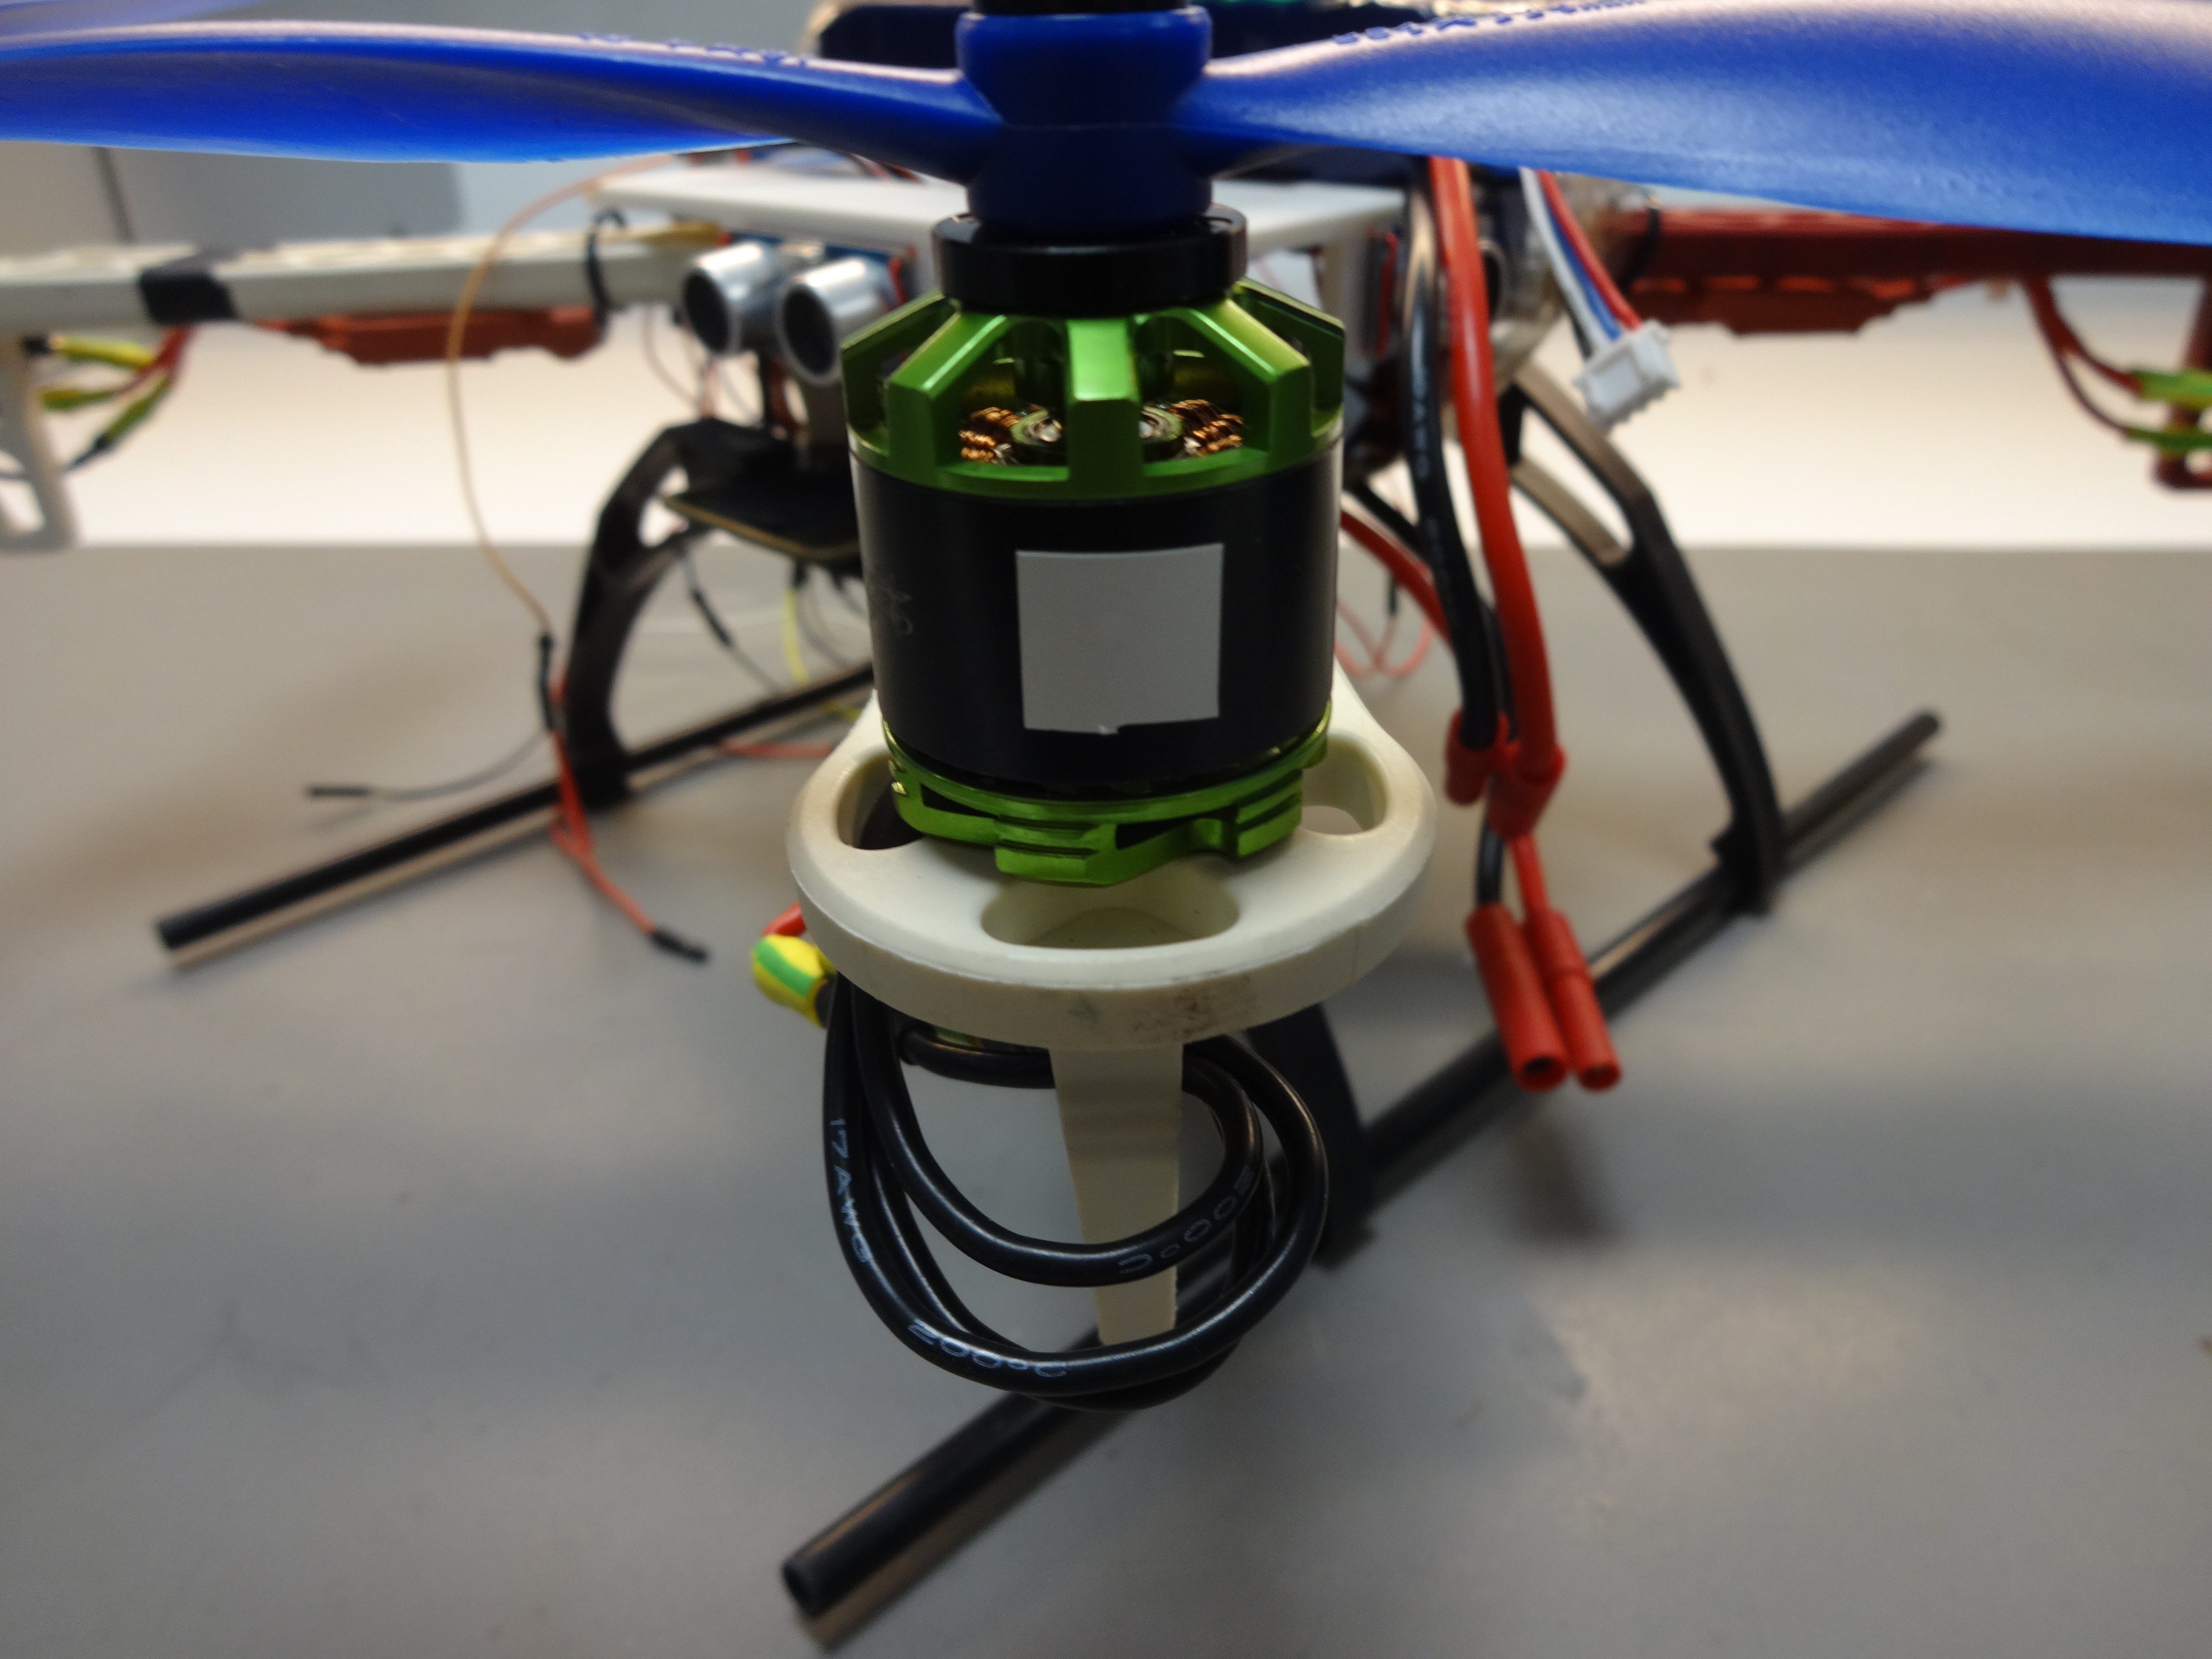
\includegraphics[width=0.5\textwidth]{images/tachometer.jpg}
	\caption{Reflective paper on the motor}
	\label{tachometer}
\end{figure}

By sending the maximum signal from the board, the RPM was measured to be 10812, with a small possible error.
In conclusion, the motors' $K_v$ coefficient found in the datasheet is in fact correct.

\subsection{APM Output and Motor Speed Relationship}

In order to use the board's output signal as an input in a mathematical model, it is necessary to find an equation to translate it into an angular rate.
First, an equation has been found that describes the relationship between motor's RPM, ESC's output signal frequency and number of motor poles \cite{RPMEq}:

\begin{equation}
\label{voltage1}
	RPM = \frac{120\times f}{n}
\end{equation}
Here, $f$ is the frequency and $n$ is the number of poles (in the case of this project - 14).

Therefore, it is possible to measure the frequency at various output values, which can then be used to define an equation that uses the board's signal length as an input value and results in an RPM.

The frequency was measured using an (NAME) oscilloscope and by connecting the probe's ground clip to the ground of the battery and the probe tip to any one of the wires between motor and the ESC. Then, by providing different output signals from the flight controller, the frequency was measured on the oscilloscope screen. An on-board filter was used to filter out some noise, especially at lower output signals. The recorded frequency was later converted into RPM using equation \ref{voltage1}, for later comparison. The output signal lengths and the corresponding frequencies converted into RPM can be seen in table \ref{FreqTable}.

\begin{table}[H]
\centering
\begin{tabular}{|c|c|}
\hline
$Output,\mu s$ 	& $RPM$ \\ \hline
762 			& 2825  \\ \hline
770				& 3189	\\ \hline
780				& 3689	\\ \hline
790				& 4211	\\ \hline
800 			& 4683  \\ \hline
810 			& 5161	\\ \hline
820 			& 5546  \\ \hline
830				& 5874 	\\ \hline
840				& 6223	\\ \hline
850 			& 6532	\\ \hline
860 			& 6795	\\ \hline
870 			& 7008	\\ \hline
880 			& 7301	\\ \hline
890 			& 7534	\\ \hline
900 			& 7730	\\ \hline
925 			& 8233	\\ \hline
950 			& 8552	\\ \hline
975 			& 8786	\\ \hline
1000 			& 9129	\\ \hline
1050 			& 9566	\\ \hline
1100 			& 9814	\\ \hline
1150 			& 10071	\\ \hline
1200			& 10260	\\ \hline
\end{tabular}
\caption{Frequency measured at ESC output, converted into RPM}
\label{FreqTable}
\end{table}

While measuring, it was observed that the frequency would never reach a steady-state and therefore, a sizeable error is possible between measurements. Because of that, RPM was manually measured using the tachometer at same output values, as seen in table \ref{RPMTable}.

\begin{table}[H]
\centering
\begin{tabular}{|c|c|}
\hline
$Output,\mu s$ 	& $RPM$ \\ \hline
762 			& 2754	\\ \hline
770				& 3170	\\ \hline
780				& 3664	\\ \hline
790				& 4210	\\ \hline
800 			& 4715  \\ \hline
810 			& 5223	\\ \hline
820 			& 5617  \\ \hline
830				& 5965 	\\ \hline
840				& 6285	\\ \hline
850 			& 6578	\\ \hline
860 			& 6846	\\ \hline
870 			& 7100	\\ \hline
880 			& 7368	\\ \hline
890 			& 7555	\\ \hline
900 			& 7790	\\ \hline
925 			& 8265	\\ \hline
950 			& 8614	\\ \hline
975 			& 8910	\\ \hline
1000 			& 9160	\\ \hline
1050 			& 9576	\\ \hline
1100 			& 9860	\\ \hline
1150 			& 10089	\\ \hline
1200			& 10261	\\ \hline
\end{tabular}
\caption{RPM measured at different values}
\label{RPMTable}
\end{table}

While measuring with tachometer, the error appeared to be less significant.

The two tables \ref{RPMTable} and \ref{FreqTable} were then plotted to see the difference, which is seen in figure \ref{RPMvsFreq}.

\begin{figure}[H]
  \centering
    \includegraphics[width=1\textwidth]{images/RPMvsFreq.png}
	\caption{Plotted values of manually measured and frequency-based RPM}
	\label{RPMvsFreq}
\end{figure}

From the plotted graphs, it can be seen that the difference is very much noticeable, especially at certain points. Due to the fact that measurements with tachometer provided smaller errors than measurements with an oscilloscope, it was decided to use the values measured with the tachometer for later calculations.

In order to make use of these findings, the RPM values have to be converted into $rad/s$ for use as angular rate. The conversion equation is:
\begin{equation}
\label{RPMConvert}
	\omega = \frac{2\pi \times RPM}{60}
\end{equation}

The values measured with tachometer were then converted into $rad/s$ and plotted on a Microsoft Excel 2010. Then, by utilising the "Format Trendline" function, a 4\textsuperscript{th} order polynomial equation fitting the original graph was obtained. The values and graphs can be seen in figure \ref{RadsTrendline}.

\begin{figure}[H]
  \centering
    \includegraphics[width=1\textwidth]{images/RadsTrendline.png}
	\caption{Converted and plotted RPM values and the trendline}
	\label{RadsTrendline}
\end{figure}

This equation, $y = -0.0000000355255899575109x^4 + 0.000154393052552121x^3 - 0.252970851547635x^2 + 185.821111008258x - 50759.3409352418$, can then be used to approximately convert the signal sent out by the flight controller in $\mu s$ into angular rate.

\section{Electronic Speed Controllers}

...

\subsection{Calibrating and Programming ESCs}
ESCs have 5 input pins, 3 of which come from the flight controller. These 3 wires supply the signal for the ESC to translate into the angle of the shaft for the motor. Before ESCs can be used, they need to be properly calibrated. Programming additional settings is optional, but in most cases necessary too. Normally, the calibration for UAVs is done by setting the throttle to full on the radio controller before powering the ESCs. However, since the board translates the throttle signal into a PWM signal, it is possible to calibrate and run the motors directly from the flight controller by sending a PWM signal using software.

The calibration is done by first sending the maximum length of signal the user wishes to use. The ESC emits sounds that are brand-specific and indicate whether the signal was successfully recognised or not. Once the maximum signal is accepted, the user the emits the minimum signal and waits for approval. Additional sound is then emitted, indicating that the calibration was successful.

Using Arduino's Servo library, a self-explanatory built-in function \textit{servo.writeMicroseconds(int value)} is used to send the signal. By default, the library has the minimum signal set to 544$\mu s$ and the maximum - to 2400$\mu s$. For this project, we shortened the range down to 700$\mu s$ and 2000$\mu s$ for both signals respectively. A commented code used to calibrate the ESC connected to the first pin of the board can be seen in listing \ref{code:calib}.

\lstinputlisting[language=C++, caption={Calibrating the ESC}, label={code:calib}]{Arduino/ESCCalib/ESCCalib.ino}

Programming additional settings of the ESC is done in a similar manner - by sending minimum and maximum signals after the ESC emits particular sounds, indicating wanted selections. The programmable features and selections are brand-specific and can be found in the datasheets. For the purposes of this project, the ESCs have been programmed to include two features - brake mode off and selection of li-ion battery.


